\chapter{Formule di quadratura}
	\label{chapterFormuleQuadratura}
	\minitoc \mtcskip
	\lettrine{I}{}n questo capitolo analizziamo il problema del calcolo di un \textbf{integrale definito},
	\begin{equation}
		\label{integrale}
		I(f)=\int_{a}^{b}f(x)dx,\qquad a<b,
	\end{equation}
	con $[a,b]$ intervallo \textit{limitato} ed $f(x)$ funzione abbastanza \textit{regolare} (cio� che non presenta singolarit�, ovvero punti di discontinuit�, nell'intervallo). Quindi nel seguito assumeremo che $f(x)$ sia \textit{continua} in $[a,b]$.\\
	Tutti i metodi descritti si basano sull'approssimazione della funzione da integrare tramite una funzione polinomiale o una funzione polinomiale a tratti.\\
	Studiamo innanzitutto il condizionamento del problema (\ref{integrale}), ovvero il problema in cui si calcola l'integrale esatto, dove si ha la perturbazione sulla funzione integranda $f(x)$, indicando con $\tilde{f}(x)$ la funzione perturbata. Ricordando allora la definizione di norma (\ref{normaC0}), si ha:\\[1cm]
	\begin{align*}
		|I(f)-I(\tilde{f})| &= |\int_{a}^{b}f(x)dx - \int_{a}^{b}\tilde{f}(x)dx| = |\int_{a}^{b}(f(x)-\tilde{f}(x))dx| \leq\\
		&\leq \int_a^b |f(x)-\tilde{f}(x)|dx  \footnoteOP{\leq} ||f-\tilde{f}||\int_a^b dx  \footnoteOP{=} [x]_a^b||f-\tilde{f}|| =\\
		&= (b-a)||f-\tilde{f}||.
	\end{align*}
	%-------- FOOTNOTES --------
	\addtocounter{footnote}{-1}
	\footnotetext{Per la disuguaglianza triangolare, in quanto l'integrale rappresenta una somma, quindi il valore assoluto dell'integrale � minore o uguale dell'integrale del valore assoluto (esattamente come una sommatoria).}
	\stepcounter{footnote}
	\footnotetext{Per definizione di norma (vedi (\ref{normaC0})), che risulta essere uno scalare (e quindi estraibile dall'integrale).}
	%-------- end FOOTNOTES --------
	
	Considerando che $|I(f)-I(\tilde{f})|$ rappresenta l'errore commesso sulla soluzione del problema e $||f-\tilde{f}||$ rappresenta una maggiorazione dell'errore commesso sui dati iniziali, si ottiene che la quantit�
	\begin{equation}
		\label{kappa}
		k=b-a
	\end{equation}
	definisce il \textit{numero di condizionamento} del problema (\ref{integrale}).

	
	\section{Formule di Newton-Cotes}
		Supponiamo di approssimare la funzione integranda $f(x)$ con un polinomio interpolante su $n+1$ ascisse equidistanti (ovvero uniformemente distribuite sull'intervallo $[a,b]$), ovvero un polinomio tale che
		$$p(x_i)=f(x)\equiv f_i,\qquad i=0,1,\dots,n,$$
		con
		\begin{equation}
			\label{partizioneUniforme}
			x_i=a+ih,\qquad h=\frac{b-a}{n}.
		\end{equation}
		Considerando adesso la forma di Lagrange (vedi (\ref{lagrange}) e (\ref{formaLagrange}) del polinomio interpolante:\\[1cm]
		\begin{align}
			I_n(f) &\approx \int_a^b p(x) dx = \int_a^b \sum_{k=0}^n f_k L_{k,n}(x) dx =\notag\\
			&= \sum_{k=0}^n f_k \int_a^b L_{k,n}(x) dx = \sum_{k=0}^n f_k \int_a^b \mathlarger\prod_{
				\begin{subarray}{c}
					j=0\\
					j\neq k
				\end{subarray}
				}^{n}\frac{x-x_j}{x_k-x_j} dx =\notag\\
			&= \sum_{k=0}^n f_k \int_0^n \mathlarger\prod_{
				\begin{subarray}{c}
					j=0\\
					j\neq k
				\end{subarray}
				}^{n}\frac{t-j}{k-j} h\cdot dt \footnoteOP{=} h\sum_{k=0}^n f_k \int_0^n \mathlarger \prod_{\begin{subarray}{c}
					j=0\\
					j\neq k
				\end{subarray}
				}^{n}\frac{t-j}{k-j} dt \notag\\
			\label{newtonCotes}
			&= \frac{b-a}{n}\sum_{k=0}^n c_{k,n}f_k,
		\end{align}
		%-------- FOOTNOTES --------
		\addtocounter{footnote}{0}
		\footnotetext{� stato effettuato il cambio di variabile $x=a+ht$, che, derivando, implica $dx=h\cdot dt$ ed il cambio di indici (infatti per avere $x\in[a,b]$ si ha $t\in[0,n]$).}
		%-------- end FOOTNOTES ----------
		
		dove
		\begin{equation}
			\label{coefficientiNewtonCotes}
			c_{k,n}=\int_0^n \mathlarger\prod_{
				\begin{subarray}{c}
					j=0\\
					j\neq k
				\end{subarray}
				}^{n}\frac{t-j}{k-j} dt, \qquad k=0,\dots,n,
		\end{equation}
		con $I_n(f)$ che rappresenta l'integrale definito tra $a$ e $b$ di $f(x)$ utilizzando un'approssimazione di $f$ tramite un polinomio interpolante su $n$ ascisse equidistanti. La (\ref{newtonCotes}) definisce quindi la generica \textbf{formula di quadratura di Newton-Cotes}.\\
		Si osserva che avendo eseguito il cambio di variabile in $t$, i coefficienti $c_{k,n}$ non dipendono pi� dall'intervallo $[a,b]$, ma soltanto dal numero $n$ (ovvero il numero di sottointervalli), in quanto quello che viene preso in considerazione sono le distanze reciproche tra le ascisse che, essendo equidistanti, risulteranno (per uno stesso $n$) sempre alla stessa distanza relativa.\\
		A seconda di quante ascisse vengono utilizzate per l'approssimazione della funzione si hanno differenti istanze della formula di Newton-Cotes generica. In particolare:
		\begin{itemize}
			\item \textbf{\underline{formula dei trapezi}:} $n=1$\\
				In questo caso abbiamo che $c_{0,1}=c_{1,1}=\sfrac{1}{2}$, infatti
				\begin{align*}
					&c_{0,1}=\int_0^1\frac{t-1}{0-1}dt=\int_0^1 dt -\int_0^1 t\;dt=1-\frac{1}{2}=\frac{1}{2},\\
					&c_{1,1}=\int_0^1\frac{t-0}{1-0}dt=\int_0^1 t\;dt = \frac{1}{2},
				\end{align*}
				e la formula dei trapezi risulta essere
				\begin{equation}
					\label{trapezi}
					I_1(f)=\frac{b-a}{2}(f(a)+f(b)).
				\end{equation}
				Il nome della formula deriva dal fatto che l'area calcolata con questo metodo coincide con l'area del trapezio avente come vertici $(a,0)$, $(a,f(a))$, $(b,f(b))$ e $(b,0)$.
			\item \textbf{\underline{formula di Simpson}:} $n=2$\\
				Si pu� facilmente verificare che in questo caso i coefficienti risultano valere
				$$c_{0,2}=c_{2,2}=\sfrac{1}{2},\quad c_{1,2}=\sfrac{4}{3},$$
				e la formula � definita da
				\begin{equation}
					\label{simpson}
					I_2(f)=\frac{b-a}{6}(f(a)+4f\left(\frac{a+b}{2}\right)+f(b)).
				\end{equation}
		\end{itemize}
		In generale si osserva che per $n\leq 6$ si hanno tutti i $c_{k,n}\geq 0$. Al contrario per $n\geq 7$ compaiono dei coefficienti negativi, che influiranno sul condizionamento del problema.
		\begin{teo}
			\label{teoCoeffNewtonCotes}
			Riguardo ai coefficienti (\ref{coefficientiNewtonCotes}) vale il seguente risultato:
			$$\frac{1}{n}\sum_{k=0}^n c_{k,n}=1.$$
		\end{teo}
		Possiamo adesso studiare il condizionamento del problema del calcolo della formula (\ref{newtonCotes}):
		\begin{align*}
			|I_n(f)-I_n(\tilde{f})| &= \frac{b-a}{n}|\sum_{k=0}^n(f_k-\tilde{f}_k)c_{k,n}| \leq \frac{b-a}{n}\sum_{k=0}^n|f_k-\tilde{f}_k|\cdot|c_{k,n}| \leq \footnotemark\\
			& \leq \left(\frac{b-a}{n}\sum_{k=0}^n|c_{k,n}|\right)||f-\tilde{f}||,\footnotemark
		\end{align*}
		%-------- FOOTNOTES --------
		\addtocounter{footnote}{-1}
		\footnotetext{Per la disuguaglianza triangolare.}
		\stepcounter{footnote}
		\footnotetext{Per la definizione di norma in $C^{(0)}$ (vedi (\ref{normaC0})).}
		%-------- end FOOTNOTES ----------
		
		Quindi si conclude che
		$$k_n=\frac{b-a}{n}\sum_{k=0}^n|c_{k,n}|$$
		� il \textit{numero di condizionamento} delle formule di Newton-Cotes.\\
		Allora, per quanto osservato prima e per il Teorema \ref{teoCoeffNewtonCotes} risulta che:
		\begin{align*}
			&k_n\equiv k, \quad n=1,\dots,6,\\
			&k_n>k, \quad n\geq 7,
		\end{align*}
		ovvero le formule di Newton-Cotes sono convenientemente utilizzabili fino ad $n=6$ (ovvero $7$ ascisse di interpolazione).

	\section{Errore e formule composite}
		Studiamo adesso l'\textit{errore di quadratura} commesso nell'utilizzare un'approssimazione polinomiale della funzione integranda al posto della funzione esatta. Ricordando la stima fatta sull'errore di interpolazione nelle (\ref{erroreInterpolazione}) e (\ref{espressioneErroreInterpolazione}) abbiamo:
		\begin{align}
			E_n(f)&=I(f)-I_n(f)=\int_a^bf(x)\;dx-\int_a^bp_n(x)\;dx=\int_a^b(f(x)-p_n(x))\;dx\notag\\
			\label{erroreQuadratura}
			&= \int_a^be(x)\;dx = \int_a^bf[x_0,\dots,x_n,x]w_{n+1}(x)\;dx.
		\end{align}
		\begin{teo}
			\label{teoErroreQuadratura}
			Se $f(x)\in C^{(n+k)}$, con
			\[
				k=\begin{cases}
					1, &\text{se $n$ � dispari},\\
					2, &\text{se $n$ � pari},
				\end{cases}
			\]
			allora l'errore di quadratura (\ref{erroreQuadratura}) � dato da
			$$E_n(f)=\nu_n\frac{f^{(n+k)}(\xi)}{(x+k)!}\left(\frac{b-a}{n}\right)^{n+k+1},$$
			per un opportuno $\xi\in[a,b]$, dove
			\[
				\nu_n=\begin{cases}
					\int_0^n \prod_{j=0}^n(t-j)\;dt, &\text{se $n$ � dispari},\\
					\int_0^n t\prod_{j=0}^n(t-j)\;dt, &\text{se $n$ � pari}.
				\end{cases}
			\]
		\end{teo}
		\begin{cor}
			Le formule definite su $n+1$ punti sono esatte per polinomi fino a grado $n$, se $n$ � dispari, e fino a grado $n+1$ se $n$ � pari.
		\end{cor}
		Quindi per il metodo dei trapezi si ha:
		\begin{equation}
			\label{erroreTrapezi}
			E_1(f)=-\frac{1}{12}f^{(2)}(\xi)(b-a)^3,\qquad\xi\in[a,b],
		\end{equation}
		mentre per il metodo di Simpson risulta:
		\begin{equation}
			\label{erroreSimpson}
			E_2(f)=-\frac{1}{90}f^{(4)}(\xi)\left(\frac{b-a}{2}\right)^5,\qquad\xi\in[a,b].
		\end{equation}

		Per poter decrementare il rapporto $\frac{b-a}{n}$ senza aumentare $n$ (per quanto detto riguardo al condizionamento del problema) si pu� utilizzare un approccio del tutto analogo a quello fatto per le \textit{spline} nel Capitolo \ref{chapterApprossimazioniFunzioni}: l'intervallo $[a,b]$ viene suddiviso in $n$ sottointervalli di uguale ampiezza e su ognuno di essi viene applicata la stessa formula di Newton-Cotes. Si ottiene cos� una \textbf{formula di Newton-Cotes composita}.\\
		Ad esempio la \textit{formula dei trapezi composita} � data dall'applicazione della formula dei trapezi su ciascun sottointervallo $[x_{i-1},x_i]$, per $i=1,\dots,n$, sulla partizione uniforme (\ref{partizioneUniforme}):
		\begin{align}
			I_1^{(n)}(f)&\equiv\frac{b-a}{n}\cdot\frac{1}{2}\left((f_0+f_1)+(f_1+f_2)+\dots+(f_{n-1}+f_n)\right)=\notag\\
			\label{trapeziComposita}
			&=\frac{b-a}{2n}\left(f_0+2\sum_{i=1}^{n-1}f_i +f_n\right),
		\end{align}
		ed il corrispondente errore di quadratura si vede valere (generalizzando il Teorema (\ref{teoErroreQuadratura})):
		\begin{equation}
			\label{erroreTrapeziComposita}
			E_1^{(n)}(f)=-\frac{n}{12}f^{(2)}(\xi)\left(\frac{b-a}{n}\right)^3,\qquad\xi\in[a,b].
		\end{equation}
		Il Codice di seguito mostra un'implementazione in \textsc{Matlab} della formula dei trapezi composita:
		\lstinputlisting[caption={Formula dei trapezi composita.}, label=lst:trapeziComposita]{code/trapeziComposita.m}
		Per la \textit{formula di Simpson composita} si ha invece (per valori pari di $n$):
		\begin{align}
			I_2^{(n)}&\equiv \frac{b-a}{3n}\left(f_0+4f_1+f_2+f_2+\dots+f_{n-2}+4f_{n-1}+f_n\right)=\notag\\
			\label{simpsonComposita}
			&=\frac{b-a}{3n}\left(4\sum_{i=1}^{n/2}f_{2i-1}+2\sum_{i=0}^{n/2}-f_0-f_n\right),
		\end{align}
		dove la prima sommatoria � per gli indici dispari mentre la seconda � per i pari ($f_0$ ed $f_n$ vengono sottratti in quanto sono contati due volte nella seconda sommatoria). Il corrispettivo errore di quadratura si vede valere:
		\begin{equation}
			\label{erroreSimpsonComposita}
			E_2^{(n)}(f)=-\frac{n}{90}f^{(4)}(\xi)\left(\frac{b-a}{n}\right)^5,\qquad\xi\in[a,b].
		\end{equation}
		\lstinputlisting[caption={Formula di Simpson composita.}, label=lst:simpsonComposita]{code/simpsonComposita.m}
		Per le due stime degli errori di quadratura sulle formule composite si vede facilmente che
		$$E_k^{(n)}(f)\rightarrow 0, \qquad n\rightarrow\infty,\qquad k=1,2.$$

	\section{Formule adattative}
		Supponiamo adesso di voler approssimare l'integrale definito di una funzione che, all'interno dell'intervallo $[a,b]$ di integrazione, ha un carattere molto variabile, ovvero ci sono punti in cui la funzione effettua rapide variazioni (per valori alti della derivata in valore assoluto) a causa di un'elevata pendenza, mentre in altri dove la funzione resta pressoch� la stessa (ovvero ha la derivata prima circa zero).\\
		In questi casi le formule composite di Newton-Cotes possono essere modificate in \textbf{formule adattative}, ovvero che sono in grado di scegliere i nodi di interpolazione a seconda dell'andamento della funzione.\\
		Ad esempio, implementando la formula dei trapezi e dei trapezi composita su due sottointervalli (che come nodi hanno $f_0$ ed $f_1$ e $f_1$ e $f_2$), si hanno i seguenti errori (vedi (\ref{erroreTrapezi}) e (\ref{erroreTrapeziComposita})):
		\begin{align*}
			&I(f)-I_1(f)\approx-\frac{1}{12}f^{(2)}(\xi)(b-a)^3,
			&I(f)-I_1^{(2)}(f)\approx-\frac{n}{12}f^{(2)}(\xi)\left(\frac{b-a}{n}\right)^3
		\end{align*}
		Quindi possiamo stimare l'errore dell'utilizzo della formula dei trapezi composita su due sottointervalli come segue:
		\begin{align*}
			&I(f)-I_1^{(2)}(f)\approx\frac{1}{4}\left(I(f)-I_1(f)\right),\\
			&\frac{3}{4}I(f)-I_1^{(2)}\approx-\frac{1}{4}I_1(f)\\
			&I(f)-I_1^{(2)}(f)\approx\frac{1}{3}\left(I_1^{(2)}(f)-I_1(f)\right),
		\end{align*}
		in modo tale che se l'errore stimato risulta maggiore di una tolleranza fissata $tol$, l'intera procedura viene reiterata su ognuno dei due sottointervalli $[a,\frac{a+b}{2}]$ e $[\frac{a+b}{2},b]$ con tolleranza $\sfrac{tol}/2$.\\
		Il Codice \ref{lst:trapeziAdattativa} mostra un'implementazione in \textsc{Matlab} della formula dei trapezi adattativa.
		\lstinputlisting[caption={Formula dei trapezi adattativa.}, label=lst:trapeziAdattativa]{code/trapeziAdattativa.m}
		In modo del tutto analogo si implementa la formula di Simpson e la formula di Simpson composita (con $n=4$, in quanto per ogni sottointervallo c'� bisogno di un punto intermedio aggiuntivo), che presentano i seguenti errori (vedi (\ref{erroreSimpson}) e (\ref{erroreSimpsonComposita})):
		\begin{align*}
			I(f)-I_2(f)\approx-\frac{1}{90}f^{(4)}(\xi)\frac{(b-a)^5}{32},\\
			I(f)-I_2^{(4)}(f)\approx-\frac{1}{90}f^{(4)}(\xi)\frac{(b-a)^5}{512},
		\end{align*}
		per poter stimare l'errore commesso con l'utilizzo della formula di Simpson composita:
		$$I(f)-I_2^{(4)}(f)\approx\frac{1}{15}\left(I_2^{(4)}-I_2(f)\right),$$
		e poter quindi procedere come visto nel caso della formula dei trapezi se l'errore stimato risulta maggiore della tolleranza fissata $tol$.
		\lstinputlisting[caption={Formula di Simpson adattativa.}, label=lst:simpsonAdattativa]{code/simpsonAdattativa.m}

	\section*{Esercizi}
		\addcontentsline{toc}{section}{Esercizi}
		\markboth{\textsc{\uppercase{Capitolo }\ref{chapterFormuleQuadratura}\uppercase{. Formule di quadratura}}}{\textsc{\uppercase{Esercizi}}}
		\begin{es} %5.1
			\label{es:5.1}
			Calcolare il numero di condizionamento dell'integrale
			$$\int_0^{e^{21}}\sin\sqrt{x}\;dx.$$
			Questo problema � ben condizionato o � malcondizionato?
		\end{es}
		\begin{sol}
			\normalfont Dalla \ref{kappa} risulta $\kappa=b-a=e^{21}-0=e^{21}>10^9$, il problema � dunque mal condizionato.
			\begin{flushright}
				\underline{Riferimenti \textsc{Matlab}}\\
				Codice \ref{lst:es5.1} (pagina \pageref{lst:es5.1})
			\end{flushright}
		\end{sol}
		\sectionline
		\begin{es} %5.2
			Derivare, dalla (\ref{coefficientiNewtonCotes}), i coefficienti della formula dei trapezi (\ref{trapezi}) e della formula di Simpson (\ref{simpson}).
		\end{es}
		\begin{sol}
			\normalfont
			\begin{itemize}
				\item Formula dei trapezi, $n=1$:
					\begin{itemize}
						\item $c_{1,1}=\int_0^1{\frac{t-0}{1-0}\:dt}=\int_0^1{t}=\left.\frac{t^2}{2}\right|_0^1=\frac{1}{2}$,
						\item $c_{0,1}=1-c_{1,1}=\frac{1}{2}$ per la (\ref{coefficientiNewtonCotes}).
					\end{itemize}
					Segue $I_1(f)=(b-a)\left(\frac{1}{2}f(a)+\frac{1}{2}f(b)\right)=\frac{b-a}{2}\left(f(a)+f(b)\right)$.
				\item Formula di Simpson, $n=2$:
					\begin{itemize}
						\item $c_{1,2}=\int_0^2{\frac{t-0}{1-0}\frac{t-2}{1-2}\:dt}=\int_2^0{t(t-2)}=\left.\left(\frac{t^3}{3}-t^2\right)\right|_0^2=\frac{4}{3}$,
						\item $c_{2,2}=\int_0^2{\frac{t-0}{2-0}\frac{t-1}{2-1}\:dt}=\int_2^0{\frac{t(t-1)}{2}}=\left.\left(\frac{t^3}{6}-\frac{t^2}{4}\right)\right|_0^2=\frac{1}{3}$,
						\item $c_{0,2}=1-c_{1,2}-c_{2,2}=\frac{1}{3}$ per la (\ref{coefficientiNewtonCotes}).
					\end{itemize}
					Segue $I_2(f)=\frac{b-a}{2}\left(\frac{1}{3}f(a)+\frac{4}{3}f\left(\frac{a+b}{2}\right)+\frac{1}{2}f(b)\right)=$\\ $=\frac{b-a}{6}\left(f(a)+4f\left(\frac{a+b}{2}\right)+f(b)\right)$.
			\end{itemize}
		\end{sol}
		\sectionline
		\begin{es} %5.3
			Verificare, utilizzando il risultato del Teorema (\ref{teoErroreQuadratura}) le (\ref{erroreTrapezi}) e (\ref{erroreSimpson}).
		\end{es}
		\begin{sol}
			\normalfont
			\begin{itemize}
				\item Formula dei trapezi, $n=1$:
					\begin{itemize}
						\item $k=1$,
						\item $\nu_1=\int_0^1{\prod_{j=0}^1{(t-j)}\:dt}=\int_0^1{(t(t-1))\:dt}=\left.\left(\frac{t^3}{3}-\frac{t^2}{2}\right)\right|_0^1=-\frac{1}{6}$.
					\end{itemize}
					Segue $E_1(f)=\nu_1\frac{f^{(2)}(\xi)}{2!}\left(\frac{b-a}{1}\right)^3=-\frac{1}{12}f^{(2)}(\xi)(b-a)^3$.
				\item Formula di Simpson, $n=2$:
					\begin{itemize}
						\item $k=2$,
						\item $\nu_2=\int_0^2{t\prod_{j=0}^2{(t-j)}\:dt}=\int_0^1{(t^2(t-1)(t-2))\:dt}=$\\$=\left.\left(\frac{t^5}{5}-3\frac{t^4}{4}+2\frac{t^3}{3}\right)\right|_0^1=-\frac{4}{15}$.
					\end{itemize}
					Segue $E_2(f)=\nu_2\frac{f^{(4)}(\xi)}{4!}\left(\frac{b-a}{2}\right)^5=-\frac{1}{90}f^{(4)}(\xi)\left(\frac{b-a}{2}\right)^5$.
			\end{itemize}
		\end{sol}
		\sectionline
		\begin{es} %5.4
			\label{es5.4}
			Scrivere una \lstinline{function} \textsc{Matlab} che implementi efficientemente la formula dei trapezi composita (\ref{trapeziComposita}).
		\end{es}
		\begin{sol}
			Si veda il Codice \ref{lst:trapeziComposita} a pagina \pageref{lst:trapeziComposita} per l'implementazione in \textsc{Matlab}.
		\end{sol}
		\sectionline
		\begin{es} %5.5
			\label{es5.5}
			Scrivere una \lstinline{function} \textsc{Matlab} che implementi efficientemente la formula di Simpson composita (\ref{simpsonComposita}).
		\end{es}
		\begin{sol}
			Si veda il Codice \ref{lst:simpsonComposita} a pagina \pageref{lst:simpsonComposita} per l'implementazione in \textsc{Matlab}. Nella soluzione proposta per unificare le due sommatorie (che corrisponderebbero a due cicli \lstinline{for}) si � portato fuori dalla seconda sommatoria il fattore $f_0$, quindi l'espressione effettivamente implementata �
			$$I_2^{(n)}(f)=\frac{b-a}{3n}(\sum_{i=1}^{n/2}(4f_{2i-1}+2f_{2i})+f_0-f_n).$$
		\end{sol}
		\sectionline
		\begin{es} %5.6
			\label{es5.6}
			Implementare efficientemente in \textsc{Matlab} la formula adattativa dei trapezi.
		\end{es}
		\begin{sol}
			Per l'implementazione della formula adattativa dei trapezi si veda il Codice \ref{lst:trapeziAdattativa} a pagina \pageref{lst:trapeziAdattativa}. L'algoritmo � stato implementato in maniera ricorsiva, utilizzando due funzioni distinte: \lstinline{trapeziAdattativa} che � la funzione di partenza e \lstinline{trapeziAdattativaRicorsiva} che � la funzione che si occupa delle ricorsioni.
		\end{sol}
		\sectionline
		\begin{es} %5.7
			\label{es5.7}
			Implementare efficientemente in \textsc{Matlab} la formula adattativa di Simpson.
		\end{es}
		\begin{sol}
			Per l'implementazione della formula adattativa di Simpson si veda il Codice \ref{lst:simpsonAdattativa} a pagina \pageref{lst:simpsonAdattativa}. L'algoritmo � stato implementato in maniera ricorsiva, utilizzando due funzioni distinte: \lstinline{simpsonAdattativa} che � la funzione di partenza e \lstinline{simpsonAdattativaRicorsiva} che � la funzione che si occupa delle ricorsioni.
		\end{sol}
		\sectionline
		\begin{es} %5.8
			\label{es:5.8}
			Come � classificabile, dal punto di vista del condizionamento, il seguente problema?
			$$\int_{\frac{1}{2}}^{100}-2x^{-3}\cos\left(x^{-2}\right)\;\mathrm{d}x\equiv\sin\left(10^{-4}\right)-\sin(4)$$
		\end{es}
		\begin{sol}
			\normalfont 
			Per la \ref{kappa} risulta $\kappa=b-a=100-1/2=99.5$, il problema � dunque mal condizionato. Visto che la funzione ha rapide variazioni in $(1,10)\subset[1/2,100]$ � preferibile utilizzare le formule di adattative invece che le formule composite; gli Esercizi 5.9 e 5.10 tabulano tali risultati.
			\begin{figure}[H]\centering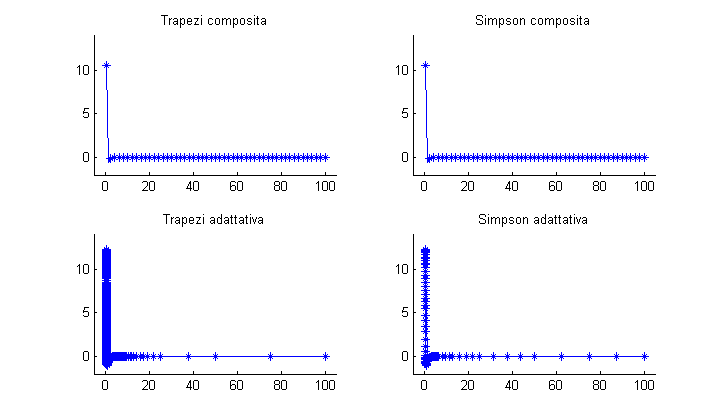
\includegraphics[scale=0.4]{es5_08.png}\end{figure}
			\begin{flushright}
				\underline{Riferimenti \textsc{Matlab}}\\
				Codice \ref{lst:es5.8} (pagina \pageref{lst:es5.8})
			\end{flushright}
		\end{sol}
		\sectionline
		\begin{es} %5.9
			\label{es:5.9}
			Utilizzare le \lstinline{function} degli Esercizi \ref{es5.4} e \ref{es5.6} per il calcolo dell'integrale $$\int_{\frac{1}{2}}^{100}-2x^{-3}\cos\left(x^{-2}\right)\;\mathrm{d}x\equiv\sin\left(10^{-4}\right)-\sin(4),$$
			indicando gli errori commessi. Si utilizzi $n=1000,2000,\dots,10000$ per la formula dei trapezi composita e $tol=10^{-1},10^{-2},\dots,10^{-5}$ per la formula dei trapezi adattativa (indicando anche il numero di punti).
		\end{es}
		\begin{sol}
			\normalfont
			$ $\\
			\begin{center}\begin{tabular}{c|c|c}
			\hline\multicolumn{3}{c}{Formula composita dei trapezi}\\\hline
			$n$ & $I$ & $E_1^{(n)}$\\\hline
			 1000&6.6401e-001&9.2897e-002\\
			 2000&7.3077e-001&2.6131e-002\\
			 3000&7.4507e-001&1.1836e-002\\
			 4000&7.5020e-001&6.7007e-003\\
			 5000&7.5260e-001&4.3009e-003\\
			 6000&7.5391e-001&2.9914e-003\\
			 7000&7.5470e-001&2.1998e-003\\
			 8000&7.5522e-001&1.6853e-003\\
			 9000&7.5557e-001&1.3321e-003\\
			 10000&7.5582e-001&1.0793e-003
			\end{tabular}\end{center}
			\begin{center}
			\begin{tabular}{c|c|c|c}
			\hline\multicolumn{4}{c}{Formula dei trapezi adattativa}\\\hline
			$tol$ & $I$ & $E_1^{(n)}$ & punti\\\hline
			  1.0e-001&7.5143e-001&5.4696e-003&159\\
			  1.0e-002&7.5563e-001&1.2676e-003&471\\
			  1.0e-003&7.5657e-001&3.3005e-004&1567\\
			  1.0e-004&7.5684e-001&6.5936e-005&4851
			\end{tabular}\end{center}
			\begin{flushright}
				\underline{Riferimenti \textsc{Matlab}}\\
				Codice \ref{lst:es5.9} (pagina \pageref{lst:es5.9})
			\end{flushright}
		\end{sol}
		\sectionline
		\begin{es} %5.10
			\label{es:5.10}
			Utilizzare le \lstinline{function} degli Esercizi \ref{es5.5} e \ref{es5.7} per il calcolo dell'integrale $$\int_{\frac{1}{2}}^{100}-2x^{-3}\cos\left(x^{-2}\right)\;\mathrm{d}x\equiv\sin\left(10^{-4}\right)-\sin(4),$$
			indicando gli errori commessi. Si utilizzi $n=1000,2000,\dots,10000$ per la formula di Simpson composita e $tol=10^{-1},10^{-2},\dots,10^{-5}$ per la formula di Simpson adattativa (indicando anche il numero di punti).
		\end{es}
		\begin{sol}
			\normalfont
			$ $\\
			\begin{center}\begin{tabular}{c|c|c}
			\hline\multicolumn{3}{c}{Formula composita di Simpson}\\\hline
			$n$ & $I$ & $E_1^{(n)}$\\\hline
			 1000 	  &7.0132e-001 	  &5.5580e-002\\
			 2000 	  &7.5303e-001 	  &3.8753e-003\\
			 3000 	  &7.5617e-001 	  &7.2977e-004\\
			 4000 	  &7.5668e-001 	  &2.2403e-004\\
			 5000 	  &7.5681e-001 	  &9.0209e-005\\
			 6000 	  &7.5686e-001 	  &4.3062e-005\\
			 7000 	  &7.5688e-001 	  &2.3094e-005\\
			 8000 	  &7.5689e-001 	  &1.3479e-005\\
			 9000 	  &7.5689e-001 	  &8.3892e-006\\
			 10000 	  &7.5690e-001 	  &5.4921e-006
			\end{tabular}\end{center}\begin{center}
			\begin{tabular}{c|c|c|c}
			\hline\multicolumn{4}{c}{Formula di Simpson adattativa}\\\hline
			$tol$ & $I$ & $E_1^{(n)}$ & punti\\\hline
			 1.0e-001 	  &7.5701e-001 	  &1.1164e-004 	  &49\\
			 1.0e-002 	  &7.5671e-001 	  &1.9384e-004 	  &65\\
			 1.0e-003 	  &7.5690e-001 	  &4.8068e-006 	  &93\\
			 1.0e-004 	  &7.5688e-001 	  &1.7808e-005 	  &181\\
			 1.0e-005 	  &7.5690e-001 	  &4.8337e-006 	  &309
			\end{tabular}\end{center}
			\begin{flushright}
				\underline{Riferimenti \textsc{Matlab}}\\
				Codice \ref{lst:es5.10} (pagina \pageref{lst:es5.10})
			\end{flushright}
		\end{sol}
	\section*{Codice degli esercizi}
		\addcontentsline{toc}{section}{Codice degli esercizi}
		\markboth{\textsc{\uppercase{Capitolo }\ref{chapterFormuleQuadratura}\uppercase{. Formule di quadratura}}}{\textsc{\uppercase{Codice degli esercizi}}}
		\lstinputlisting[caption={Esercizio \ref{es:5.1}.}, label=lst:es5.1]{code/es5_1.m}
		\sectionline
		\lstinputlisting[caption={Esercizio \ref{es:5.8}.}, label=lst:es5.8]{code/es5_8.m}
		\sectionline
		\lstinputlisting[caption={Esercizio \ref{es:5.9}.}, label=lst:es5.9]{code/es5_9.m}
		\sectionline
		\lstinputlisting[caption={Esercizio \ref{es:5.10}.}, label=lst:es5.10]{code/es5_10.m}
		